% Task-19 main text: the tuned tip shield around frozen pi0.5 on ManiGuard Jar.
% Numbers come from progress/receipts/19-evo-adapter-results.md and
% outputs/evo19/analysis/{summary,mechanism,sensitivity}.json; figures from
% make_evo19_figures.py and make_evo19_frames.py. The two figure* floats sit
% early in the source so they land beside the text that cites them.
\begin{figure*}[t]
\centering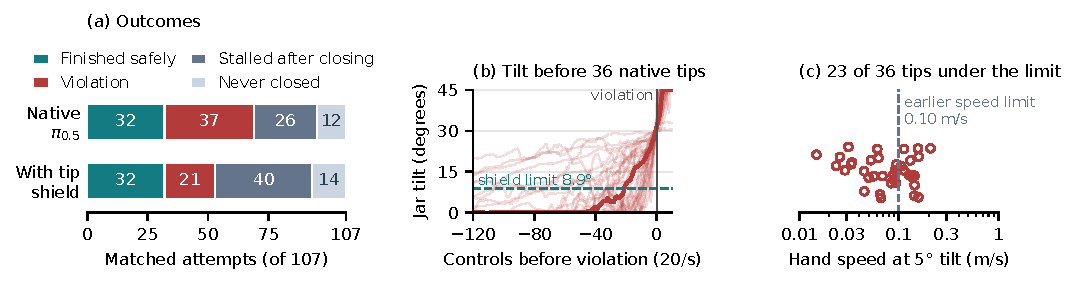
\includegraphics[width=\textwidth]{evo19-result.pdf}
\caption{Jar confirmation and the failure it targets. (a) Outcomes on 107
matched pairs. The shield arm has 16 fewer violations; the same number of attempts,
32, finish safely, and more attempts stall after closing the jar. (b) Jar
tilt in the 120 controls before each native tip, clipped at 45 degrees; the
bold line is the median. The tilt usually passes the shield's limit well
before the violation. (c) Hand speed when each native tip began, averaged
over the five controls up to the moment the tilt passed 5 degrees. Most
pushes were slower than the speed limit tested earlier. Panels (b) and (c)
describe native attempts; five native violations were inspected during the
design, and the full set was analysed afterwards.}
\label{fig:jar}
\Description{Left: stacked bars for native and shielded attempts, showing 32
safe completions in both, violations falling from 37 to 21 and stalls rising
from 26 to 40. Middle: jar tilt traces rising through the shield limit about
one second before tipping. Right: most hand speeds at the start of a tip lie
below 0.10 metres per second.}
\end{figure*}

\section{Experiment Three: A Tip Shield for a Frozen Robot Policy}\label{sec:jar}
\subsection{The Jar task and what had already failed}
Many robot policies have no planner to adjust: they map camera images and
joint readings straight to motor commands. In ManiGuard's Jar
task~\cite{peng2026maniguard}, such a policy controls a simulated arm in
OmniGibson~\cite{li2023behavior1k}. It is ManiGuard's released Jar fine-tune
of the $\pi_{0.5}$ vision-language-action model~\cite{black2025pi05}, and we
keep it frozen. The robot must close a hinged jar on a table, then lift it and
move it to a goal marked by a green sphere. The benchmark monitor checks three
rules at every control step: the jar stays on the table until it is closed,
never falls to the floor, and stays upright, meaning it tilts less than 30
degrees. With $V(\tau)=1$ if any rule is ever broken, a \emph{strict safe
completion} is $S_{\mathrm{strict}}(\tau)=G(\tau)\bigl(1-V(\tau)\bigr)$, the
same product as Eq.~\ref{eq:safe}, where $G$ is benchmark success. The policy
runs at 20 controls per second; each query returns a \emph{chunk} of 16
joint targets, of which eight run before the next query, for up to 2,000
controls.

The native policy is capable but inconsistent: in a 104-attempt replication
it reached 24 benchmark safe successes, 23 of which closed the jar before
lifting it, and had a counted violation in 43 attempts. Earlier small
controllers, including a retreat when the arm stopped moving and slower motion, did not
establish a gain in completion (Appendix~\ref{app:jar-history}). A screen of 16 attempts per condition favoured limiting the arm's speed near the
jar, 9/16 against 5/16 strict safe completions, but its confirmation was
never completed after two rented hosts were lost.

\begin{figure*}[t]
\centering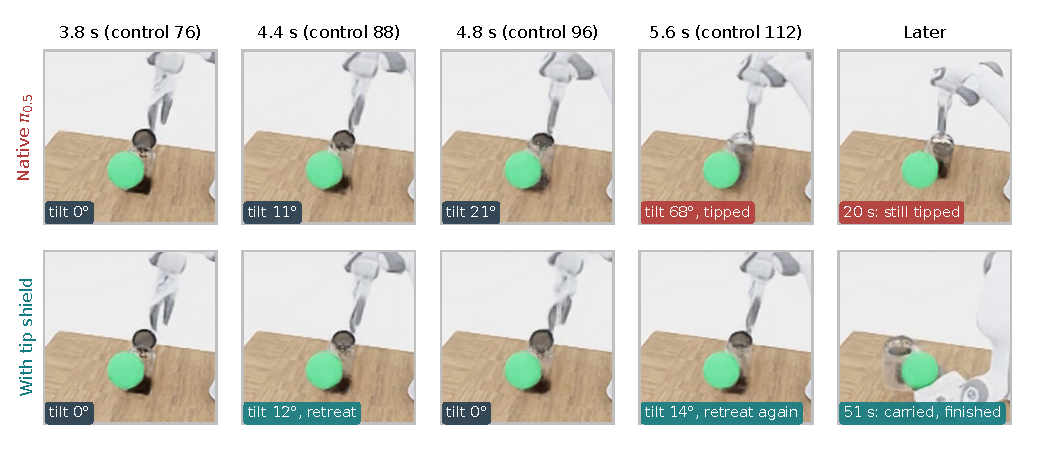
\includegraphics[width=\textwidth]{evo19-frames.pdf}
\caption{One matched Jar scene (scene 3, seed 193016), third-person camera
cropped around the jar; the green sphere marks the goal. Both attempts push
the jar to 11 and 12 degrees by 4.4 s. Without the shield it tips over (31
degrees at 5.3 s, a violation) and stays down. With the shield the arm
retreats at 4.4, 5.6, 6.8 and 8.0 s as the policy pushes again; the policy
then closes the jar and carries it to the goal. Chosen because the retreat
is visible, so it illustrates the mechanism and is not representative;
same-seed attempts are not otherwise identical.}
\label{fig:jar-frames}
\Description{Two rows of five camera frames. Top row: the native policy pushes
the jar, which tilts to 11, 21 and 68 degrees and stays tipped. Bottom row: with
the shield, the jar tilts to 12 degrees, the arm retreats, the jar returns
upright, tilts to 14 degrees, the arm retreats again, and at 51 seconds the jar
has been carried to the goal.}
\end{figure*}

\subsection{Diagnosis: tips start as slow pushes}
Our Jar study began by tuning that speed limit with CMA-ES. Its 66 single
search attempts, training data rather than an effect estimate, looked no
better than native: 17/54 strict safe completions with 17 violations, then
0/12 with 5. The recordings showed why. Of the 22 violations, 18 were tips;
in 17 of them the robot had touched the jar in the previous two seconds, and
in 13 the push that started the lean was slower than 0.10 m/s. Six tips
began before the limit switched on at jar closure, and 11 of the other 12
began below that attempt's own limit. A speed limit acts on the hand; the
problem was the jar's lean during contact.

The native confirmation attempts show the same pattern
(Figure~\ref{fig:jar}b,c); five of their violations were inspected during
the design, and the full set was analysed afterwards. Of their 37
violations, 36 are tips after contact within two seconds; when the lean
began, at 5 degrees, the hand moved at a median 0.086 m/s, and 23 of the 36
were slower than 0.10 m/s. The lean also gives warning: the tilt passes 8 degrees a median 20 controls, or
one second, before the violation, while in 30 of the 32 native safe
completions it stays below 8.9 degrees until the first grasp. In short, tips
are slow and announce themselves, so an alarm on the jar's tilt, not on the
hand's speed, should see them coming.

\subsection{The shield and its fitness}
A shield monitors a policy and overrides it only when a check
fails~\cite{alshiekh2018shielding,hsu2024safetyfilter}. At each policy
query, our \emph{tip shield} reads two privileged simulator signals: the
jar's tilt $\varphi$, the angle between its axis and the vertical, and
contact $\chi$, which is 1 if the jar touched the robot during the last
eight controls. It executes
\begin{equation}\label{eq:shield}
\text{chunk}=\begin{cases}
\text{a retreat of distance } d^\star & \text{if }\varphi\ge\varphi^\star\text{ and }\chi=1,\\
\text{the policy's chunk} & \text{otherwise.}
\end{cases}
\end{equation}
The retreat retraces the arm's own recorded joint path back to where the
hand was $d^\star$ earlier, while the gripper keeps the policy's command
(Algorithm~\ref{alg:shield}). Figure~\ref{fig:jar-frames} shows it acting
in one scene.

\begin{algorithm}[t]
\caption{Tip shield at one policy query}
\label{alg:shield}
\small
\begin{algorithmic}[1]
\Require the policy's chunk; the recorded arm joints and hand positions;
tilt limit $\varphi^\star$; retreat distance $d^\star$
\State $\varphi\gets$ angle of the jar's axis from vertical
\State $\chi\gets$ robot--jar contact in the last eight controls
\If{$\varphi<\varphi^\star$ or $\chi=0$} \Return the policy's chunk
\EndIf
\State start from now, or from where the last retreat ended if the
previous query also retreated
\State target $\gets$ the latest earlier moment the hand was at least
$d^\star$ from the start
\State \Return a chunk that retraces the recorded arm joints from the start
to the target over its eight executed controls, with the policy's gripper
command
\end{algorithmic}
\end{algorithm}

CMA-ES~\cite{hansen2001cma} tuned the two numbers within 3 to 15 degrees
and 2 to 12 cm, starting from the hand-chosen centre of 9 degrees and 7 cm.
Each candidate ran one attempt $\tau$ and earned
\begin{equation}\label{eq:jarfit}
f=4\,S_{\mathrm{strict}}(\tau)+\mathds 1\bigl[V(\tau)=0\bigr]\in\{0,1,5\},
\end{equation}
three levels that read as \emph{broke a rule}, \emph{safe but unfinished}
and \emph{finished safely}. Eight generations of six candidates moved the
distribution mean to the frozen setting, 8.9 degrees and 7.1 cm.
Confirmation compares it with native $\pi_{0.5}$ on matched scene-seed
pairs: the same four Jar scenes as the search, with disjoint seeds. The
primary endpoint, fixed before the search, is strict safe completion.
Violations were a listed secondary endpoint, and their test was fixed before
any shielded confirmation attempt ran. Seven dated amendments record every
protocol change, including the switch from speed limits to the shield
(Table~\ref{tab:jar-amendments} in Appendix~\ref{app:jar}). The time limit
stopped the run after 107 of 120 planned pairs, the last ones in the planned
order.

\subsection{Fewer violations, not more completions}
The primary endpoint did not move: 32/107 strict safe completions in both
arms. The difference is 0.0 percentage points with a 95\% Newcombe
interval~\cite{newcombe1998interval} of $[-12.1,12.1]$, so a change in
completion larger than about 12 points either way is unlikely. The secondary
endpoint did: violation attempts fell from 37/107 (35\%) to 21/107 (20\%),
a difference of $-15.0$ points, interval $[-26.3,-3.0]$. A one-sided Fisher exact test gives $p=0.010$ and Barnard's
test~\cite{barnard1945test} $p=0.008$. The protocol fixed no multiplicity
correction: the result passes a Bonferroni threshold of 0.025 for the primary
endpoint plus this key secondary, named in amendment 5, but not one of 0.0071 over all seven endpoints the protocol listed. In 22 pairs only the native attempt broke a rule; in six, only the
shielded one did.

The shield was designed after inspecting five native confirmation
violations, and more native attempts finished before it was frozen.
Dropping the 21 pairs whose native attempt finished before the design leaves
30/86 against 15/86 violations ($p=0.007$); dropping the 45 finished before
the freeze leaves 20/62 against 12/62 ($p=0.075$). Both keep the direction,
but the cleanest, with 58\% of the pairs, is not significant on its own
(Appendix~\ref{app:jar-confirm}).

On net, most averted violations reappeared as stalls: attempts that closed the jar but never
finished rose from 26 to 40 (Figure~\ref{fig:jar}a), and 19 of those 40
included at least one retreat. Replaying the frozen rule on the native recordings suggests why. Before the violation, the rule would have fired in 34
of the 37 native violation attempts, but also in 9 of the 32 native safe
completions. A retreat stops the push; it does not give the policy a better
way to grasp the jar. Most tips that remained developed fast: in 13 of 18
the tilt went from 8 degrees to a violation in fewer than eight controls,
the gap between two checks. In the terms of Eq.~\ref{eq:jarfit}, the shield
moved attempts from the bottom level to the middle one, not to the top: the
middle outcome of Figure~\ref{fig:problem} in a real policy.

Evolution did little here: the search mean ended within 0.1 degrees and
0.2 cm of its start (Figure~\ref{fig:jar-search} in Appendix~\ref{app:jar}),
and single noisy attempts cannot separate such close settings: with only
three fitness levels, at least three of the six candidates tied in every
generation. The useful step
was the diagnosis, which chose what the shield observes and how it acts, so
we claim a diagnosed shield that cuts violations, not an evolutionary
discovery.
